%------------------------------------------------------------------------------
% SMURF Paper
%------------------------------------------------------------------------------

\documentclass[useAMS,usenatbib,nofootinbib]{mn2e}

% this is needed to get pdftex to work properly!
\usepackage[pdftex]{graphicx}

\usepackage{amsmath}
\usepackage{url}
\usepackage{natbib}
\usepackage{rotating}

% --- Some user defined macros ------------------------------------------------

% journals
\newcommand{\apj}{\rm ApJ}
\newcommand{\apjl}{\rm ApJL}
\newcommand{\apjs}{\rm ApJS}
\newcommand{\aaps}{\rm A$\&$AS}
\newcommand{\aap}{\rm A$\&$A}
\newcommand{\aapr}{\rm A$\&$AR}
\newcommand{\mnras}{\rm MNRAS}
\newcommand{\aj}{\rm Astron. J.}
\newcommand{\araa}{\rm ARAA}
\newcommand{\nat}{\rm Nature}
\newcommand{\pasj}{\rm PASJ}
\newcommand{\pasp}{\rm Publ. Astron. Soc. Pac.}
\newcommand{\ASP}{\rm ASP COnference Series}
\newcommand{\CASP}{\rm Comm. Astrophys. Space Phys.}
\newcommand{\astroph}{\rm astro-ph/}


% common acronyms etc.
\newcommand{\snr}{SNR}
\newcommand{\scuba}{SCUBA-2}
\newcommand{\rms}{RMS}

% these are approximately less-than and greater-than symbols
\def\lsim{\mathrel{\lower2.5pt\vbox{\lineskip=0pt\baselineskip=0pt
          \hbox{$<$}\hbox{$\sim$}}}}

\def\gsim{\mathrel{\lower2.5pt\vbox{\lineskip=0pt\baselineskip=0pt
          \hbox{$>$}\hbox{$\sim$}}}}


% ----------------------------------------------------------------------------

\title[SMURF: an iterative map-maker for SCUBA-2]{The Sub-Millimetre User
Reduction Facility: an iterative map-maker for SCUBA-2}

\author[Edward~L.~Chapin~et~al.]{
  \parbox[t]{\textwidth}{
    Edward~L.~Chapin$^{1}$\thanks{E-mail:~echapin@phas.ubc.ca},
    David~S.~Berry$^{2}$,
    Andrew~G.~Gibb$^{1}$,
    Tim~Jenness$^{2}$,
    Douglas~Scott$^{1}$
  }
  \\
  \\
  $^{1}$Dept. of Physics \& Astronomy, University of British Columbia,
  6224 Agricultural Road, Vancouver, B.C. V6T 1Z1, Canada\\
  $^{2}$JointAstronomy Centre, 660 N. A`oh\={o}k\={u} Place, University
  Park, Hilo, Hawaii 96720, USA}

\begin{document}

\label{firstpage}

\maketitle

\begin{abstract}
  We describe the properties of data from the Submillimetre Common
  User Bolometer Array 2 (SCUBA-2) taken during the Shared Risk
  Observing period from 2010 February 11 to 2010 March 25, and the
  production of maps using the Sub-Millimetre User Reduction Facility
  (SMURF). Our iterative approach is similar to those used to reduce
  data from other ground-based submillimetre telescopes in recent
  years, and recovers angular scales up to the size of the array
  footprint (approximately 2\,arcmin). The method is also able to
  achieve the theoretical white-noise limit of the instrument for
  point-source studies.
\end{abstract}


\begin{keywords}
chicken, chicken: chicken, chicken: chicken -- chicken
\end{keywords}

%------------------------------------------------------------------------------
\section{Introduction}
\label{sec:intro}
%------------------------------------------------------------------------------

\textbf{Guideline for figures:}

\begin{itemize}
\item minimize excess whitespace around the figure to optimize usage of space
\item ensure a decent line thickness
\item use a Times font for labels with a thickness that resembles the
  text in the body. The font size should be similar to the main body
  text or larger
\item avoid using colour unless it is necessary for emphasis
\end{itemize}

\textbf{start intro here...}

The Submillimetre Common User Bolometer Array 2
\citep[\scuba,][]{holland2006} is a new instrument for the 15-m
James Clerk Maxwell Telescope (JCMT) on Mauna Kea, Hawai'i. The camera
can simultaneously image the sky in two broad bands centered over 450
and 850\,\micron. Ultimately, the instrument will also be equipped
with a Fourier transform spectrometer \citep[FTS-2,][]{gom2010}, and a polarimeter
\cite[POL-2,][]{bastien2005}. This paper describes the Submillimetre User Reduction Facility,
SMURF, a software package for reducing the imaging data, with an
emphasis on data taken during the SCUBA-2 Shared-Risks Observing period
(S2SRO) which took place from 2010 February 11 to 2010 March 25. The reduction
of FTS-2 and POL-2 data will be described at a later date once these
additional instruments have been commissioned.

Over the last twenty years, the submillimetre band (defined here to be
200--1000\,\micron) has revolutionized several important areas of
astrophysics: helping to characterize the early stages of
star-formation by identifying the dense, cold regions in molecular
clouds where stars may eventually form; discovering through blind
surveys the locations and surface density of a class of massive
star-forming galaxies in the early Universe, now referred to as
submillimetre galaxies, or SMGs; and finding debris disks around
nearby stars, the early stages of planet formation.

Styles of map-making: maximum likelihood
\citep[e.g.,][]{patanchon2008}; iterative -- see \citet{johnstone2000}
implementation of \citet{wright1996} to remove chop,
\citet{kovacs2008} for SHARC-2 etc.; de-correlation using PCA analysis
\citep[e.g.][]{laurent2005,scott2008,aguirre2010}.

Since \scuba\ will ultimately have nearly 10,000 working bolometers,
considerably larger than any other existing ground, or space-spaced
bolometer cameras, SMURF has been designed to use a less accurate,
though faster and less memory-intensive iterative approach that
attempts to model and remove most of the correlated signal components,
and then regrid the residuals signals. This method is similar in
spirit to the Comprehensive Reduction Utility for SHARC-2
\citep[CRUSH,][]{kovacs2008}, and the pipeline developed for the
Bolocam Galactic Plane Survey \citep{aguirre2010}.

%------------------------------------------------------------------------------
\section{Data Properties}
\label{sec:data}
%------------------------------------------------------------------------------

My thought is that this section would give the basics about how
SCUBA-2 works, and then more specific details for the S2SRO
observations.

%--------------------------------------------------
\subsection{How \scuba\ takes measurements}
%--------------------------------------------------

Before describing the data-reduction algorithm in detail, we summarize
the basic strategy used to make measurements with SCUBA-2.

The first generation of submm bolometer cameras used NTD germanium
thermistors (e.g., SCUBA, MAMBO, BOLOCAM, AzTEC, LABOCA...).
Generally speaking, these devices are operated using a current bias;
changing thermal conditions alter their impedence, resulting in a
changing Voltage that can be measured. The bolometers are cooled so
that they are {\em background limited} -- the dominant noise term is
the optical load from sources outside of the cryostat (emissivity from
telescope, atmospheric fluctuations, and astronomical sources).

In contrast, SCUBA-2 belongs to a new generation of cameras that uses
superconducting transition-edge sensors (TESs, like ACT, SPT,
MUSTANG). These devices are held at the critical temperature,
$T_\mathrm{C}$, below which the material becomes a superconductor, and
above which it becomes a normal conductor. Within this transition,
tiny temperature fluctuations can produce huge changes in
impedence. The devices are operated with a voltage bias, so that
thermal fluctuations produce changing currents, which in turn generate
changing local magnetic fields. Chains of superconducting quantum
interference devices (SQUIDs) are used to amplify these signals,
ultimately providing a larger changing current that may be
digitized. Like the NTD thermistor-based cameras, SCUBA-2 is cooled in
order to be background limited. However, a superior over-all
sensitivity on a per-bolometer basis is achieved through its improved
responsivity (similar to an improved quantum efficiency for a CCD).

The load on the detectors can vary substantially, both from thermal
sources within and outside the SCUBA-2 cryostat. In order to operate
the camera across a broad dynamic range of conditions, it is therefore
necessary to thermally control the focal plane. This is achieved by
providing a fridge {\em base temperature}, $T_\mathrm{B}$ that is
well-below $T_\mathrm{C}$, and then using heaters that are connected
to each bolometer to place the array in to transition.

The focal plane is divided into four quadrants, each filled with 32
column $\times$ 40 row sub-arrays labelled s4a--s4d at 450\,\micron,
and s8a--s8d at 850\,\micron. To avoid independent bias and readout
wires to each bolometer, each array is multiplexed by column. There is
an additional row of dark SQUIDs with no TESs or thermal absorber used
to monitor non-thermal noise sources.

The camera has been designed so that the absolute response of each
detector can be established by ramping currents through the individual
pixel heaters to produce Joule heating power, $P_\mathrm{J} =
\epsilon I^2R$, where $I$ is the known current, $R$ is the heater
resistance, and $\epsilon$ is the efficiency with which power is
transferred to the bolometer. In order to calibrate the total factor
$\epsilon R$, SCUBA-2 posesses an internal flatfield source.

In general, bolometers have two predominant noise components: (i) the
effectively white thermal noise produced by the phonon and optical
loading on the absorbers; and (ii) and longer-timescale drift
resulting from slow variations in the mean load (e.g. fridge,
telescope, or atmospheric changes), and also the readout
electronics. As such, the spectrum corresponding to a bolometer
time-series exhibits a ``$1/f$'' shape below some knee frequency,
$f_\mathrm{knee}$, and is relatively flat at higher frequencies. Other
smaller effects may include line features in the spectrum (a common
culprit is pickup from AC mains, or microphonic signals induced by
mechanical vibrations), and finally a roll-off towards the Nyquist
frequency caused by the anti-aliasing filter that precedes
digitization.

In order to observe astronomical sources, it is clearly advantageous
that the signals appear in the region of the spectrum that offers the
highest \snr, namely frequencies above $f_\mathrm{knee}$. This effect
is achieved by modulating the signal; the original SCUBA primarily
used the JCMT chopping secondary to place sources into the spectrum at
about $\sim$10\,Hz. The problem with this strategy was that SCUBA was
ultimately limited to recovering information on angular scales smaller
than the chop throw (a maximum of a couple of arcmin)... cite
somebody. The primary approach to map-making with SCUBA-2 is instead
to slew the entire telescope at such a rate that angular scales of
interest are crossed on time scales shorter than $1/f_\mathrm{knee}$,
similar to other ground-based instruments (MAMBO, BOLOCAM, SHARC-II,
AzTEC, LABOCA,...). The desire to scan rapidly has two basic
constraints: (i) the telescope cannot physically move faster that
several hundred arcsec\,sec$^{-1}$ without requiring unacceptably
large accelerations to change direction, and (ii) bolometers are
designed with a thermal time constant that balance response with
sensitivity. Taking these constraints into consideration, SCUBA-2 was
ultimately designed to work at a maximum scan velocity of
600\,arcsec\,sec$^{-1}$. The data acquisition system has a target
sample rate of 200\,Hz, which at that scan velocity results in a
sample every 3.0\,arcsec, or approximately one third of the
450\,\micron\ diffraction-limited full-width at half-maximum (FWHM) --
a typical rule-of-thumb for adequately sampling a Gaussian point
spread function (PSF). Similarly, the SCUBA-2 bolometers are designed
to have a time constant of 2 ms \textbf{check that number!} in order
to avoid distorting PSF-sized sources at this maximum scan rate.

The scan strategy is designed, primarily, to mitigate the effects of
$1/f$ drift. The simplest scan one might use is a raster pattern, or a
series of parallel passes across this field. However, such a scan
yields extremely poor performace for structures that are transverse to
the scan direction, since a long time will have ellapsed between each
parallel step, and the signal will therefore be totally dominated by
the $1/f$ noise. In addition, other noise features may appear in the
data periodically. With such a regularly spaced periodic scan
strategy, these noise features can easily conspire with the scan
pattern to produce similarly periodic noise structures in the map, or
\emph{scan-synchronous} noise. It has therefore been recognized for
some time that scan strategies that visit each region of the map on as
many different time scales, and scan angles as possible offer the best
protection against large-scale noise (...cite some people...). As a
tradeoff between truly random scan patterns and feasibility of
implementation taking into consideration both mechanical and
scheduling constraints, SCUBA-2 presently has three primary scan
modes: PONG (cite Borys et al.), Lissajous, and Daisy... (more
citations? Kovacs et al. has a nice description... also CMB
literature).

%-------------------------------------------------
\subsection{\scuba\ shared-risk observations}
%-------------------------------------------------

The S2SRO period, as mentioned above, took place during February and
March 2010. For the purpose of this paper, we will consider data taken
as early as 2009 December 3, at which point the instrument was being
commissioned in a similar configuration to that of the S2SRO
period. At this time, each of the 450 and 850\,\micron\ focal planes
were populated with single subarrays, s4a and s8d respectively. There
were two main mechanical problems to contend with during this
period. First, the fridge was not able to cool the focal plane to the
desired base temperature of ... which affected stability, particularly
at 850\,\micron. Second, there were problems with the subarray
fabrication process which led to large numbers of dead pixels, as well
as large-scale variations in $T_\mathrm{C}$ and the thermal
conductivity, $G$. These latter issues made it difficult to
simulataneously lock all of the bolometers, and in addition many of
the bolometers that were locked did not achieve their minimum
theoretical noise performance, since it is not possible to adjust the
individual temperature biases and place each device into the optimal
region of the superconducting transition.

While there were moderate variations from night-to-night during the
observing period, there were typically 600 to 900 working detectors in
each of the s4a and s8d subarrays. Fig.~\ref{fig:sensitivities} shows
representative responsivity maps for the two subarrays from the middle
of S2SRO based on the response to ramping the bolometer heaters.

\begin{figure}
\vspace{2cm}
\textbf{This will be a figure showing s4a and s8d responsivity maps}
\vspace{2cm}
\caption{The response of each bolometer to known input heater power
  for a typical night during S2SRO. The s4a subarray had a
  particularly large variation in $T_\mathrm{C}$ towards the
  bottom-right which resulted in lower responsivity, and
  correspondingly larger noise. The s8d array also suffered
  significant variations across the focal plane, in particular
  removing larger number of useful detectors from the bottom-left.}
\label{fig:sensitivities}
\end{figure}

\subsubsection{Time series}

In Fig.~\ref{fig:bolos_mix} we show sample time series from single
bolometers in each of the subarrays, as well as variations in the
mixing chamber temperature (as a proxy for the focal-plane
temperature), and the telescope pointing during a PONG scan.

\begin{figure}
\centering
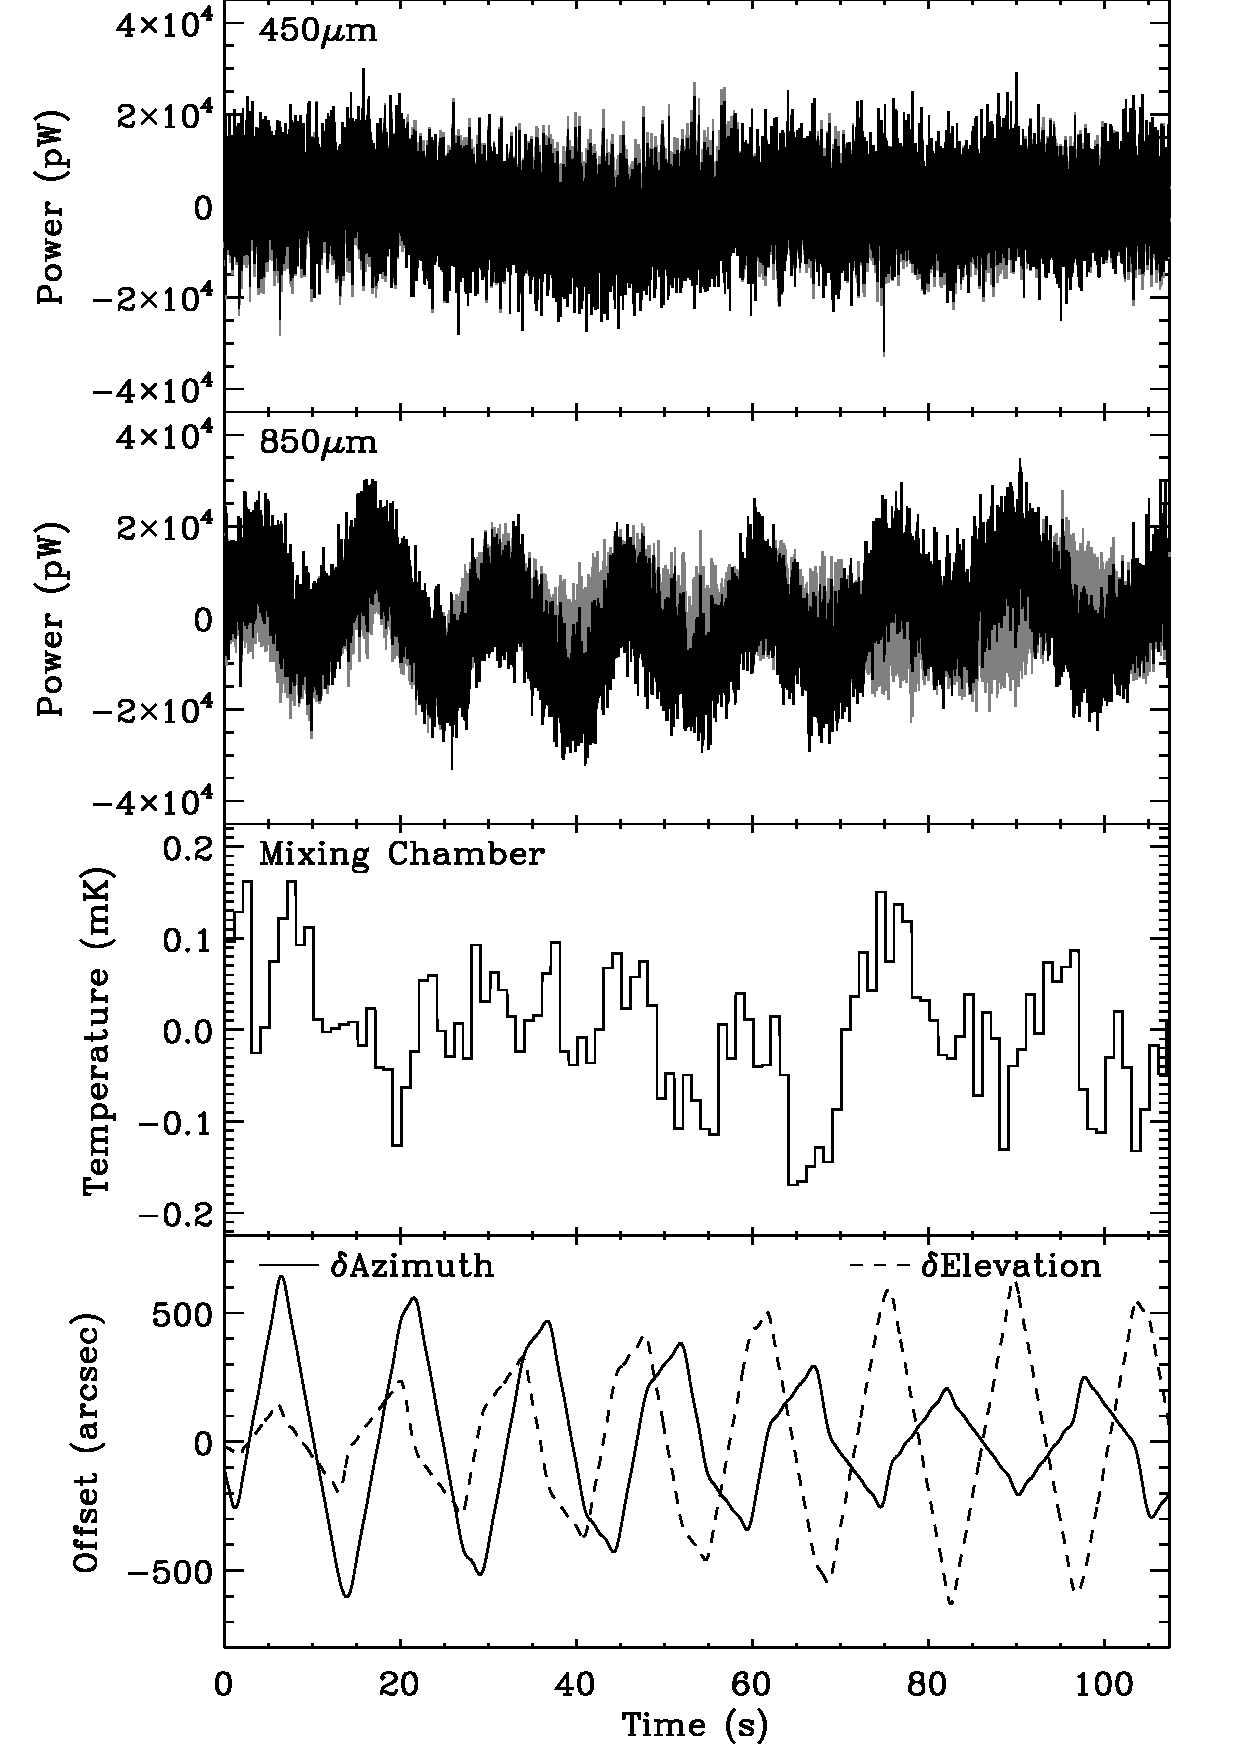
\includegraphics[width=\linewidth]{bolos_point_mix.pdf}
\caption{A comparison between single bolometer time series in each
  band (top two plots), with the mixing chamber temperature and
  azimuth/elevation pointing offsets. There is a strong correlation
  between the bolometers and the roughly $\sim$25\,s oscillation in
  the fridge, but not with the telescope motion. Also note that the
  total power in this primary signal is similar at both 450 and
  850\,\micron, pointing to an internal rather than an external
  source. The grey signals overplotted in the top-two panels show the
  residual time-series after removing the common-mode signal. This
  operation shows: (i) that most of the low-frequency signal is common
  to all of the bolometers; and (ii) the non-correlated, and
  predominantly white noise at 450\,\micron\ is significantly larger
  than at 850\,\micron.}
\label{fig:bolos_mix}
\end{figure}


Both bolometers share significant long-timescale structure
($\gsim10$\,s) that appears to be related to variations in the fridge
base temperature, although the similarity is clearly greater at
850\,\micron. In this particular case, the total power in the
fluctuations at 450\,\micron, from $-0.04$\,pW to $+0.08$, are larger
than the $-0.03$\,pW to $+0.05$\,pW fluctuations at 850\,\micron. Such
behaviour might be expected if there is a comparable varying thermal
load from the fridge at each wavelength, but a larger contribution of
astmospheric variations through the 450\,\micron\ bandpass filters. We
also note that there is no obvious strong correlation between the
low-frequency signal structure at either wavelength at the telescope
motion.

The low-frequency signal component of the bolometer signals is also
highly correlated amongst bolometers in the same subarray. We have
calculate a common-mode signal, $\mathbf{c}(t)$ as the straight
average time series of all the working bolometers. We then fit the
amplitude of $\mathbf{c}(t)$ at each wavelength to the time series
shown in Fig.~\ref{fig:bolos_mix} and remove it, yielding the grey
residual signals. These residuals are quite flat, although still with
noticeable variations. The white noise is also apparent, and larger at
450\,\micron\ as one would expect from the larger loading compared to
850\,\micron.

\subsubsection{Power spectral densities}

Next, we produce power spectral density (PSD) plots for several
representative bolometers in Fig.~\ref{fig:pspec}. To produce this
figure, we follow the convention that the PSD as a function of
frequency, $\mathbf{P}(f)$, is normalized such that the integral over
frequency gives the same variance as the time-series variance across
the full time series. In other words, given a bolometer signal
$\mathbf{b}(t)$,
%
\begin{equation}
\int \mathbf{P}(f) df = \langle\mathbf{b}^2(t)\rangle.
\end{equation}
%
However, we only show the PSD up to the Nyquist frequency, so the
conversion from variance measured in the frequency domain to the time
domain requires and additional multiplcation by 2; hence the units are
pW$^2$\,Hz$^{-1}$ rather than pW$^2$\,s.

\begin{figure}
\centering
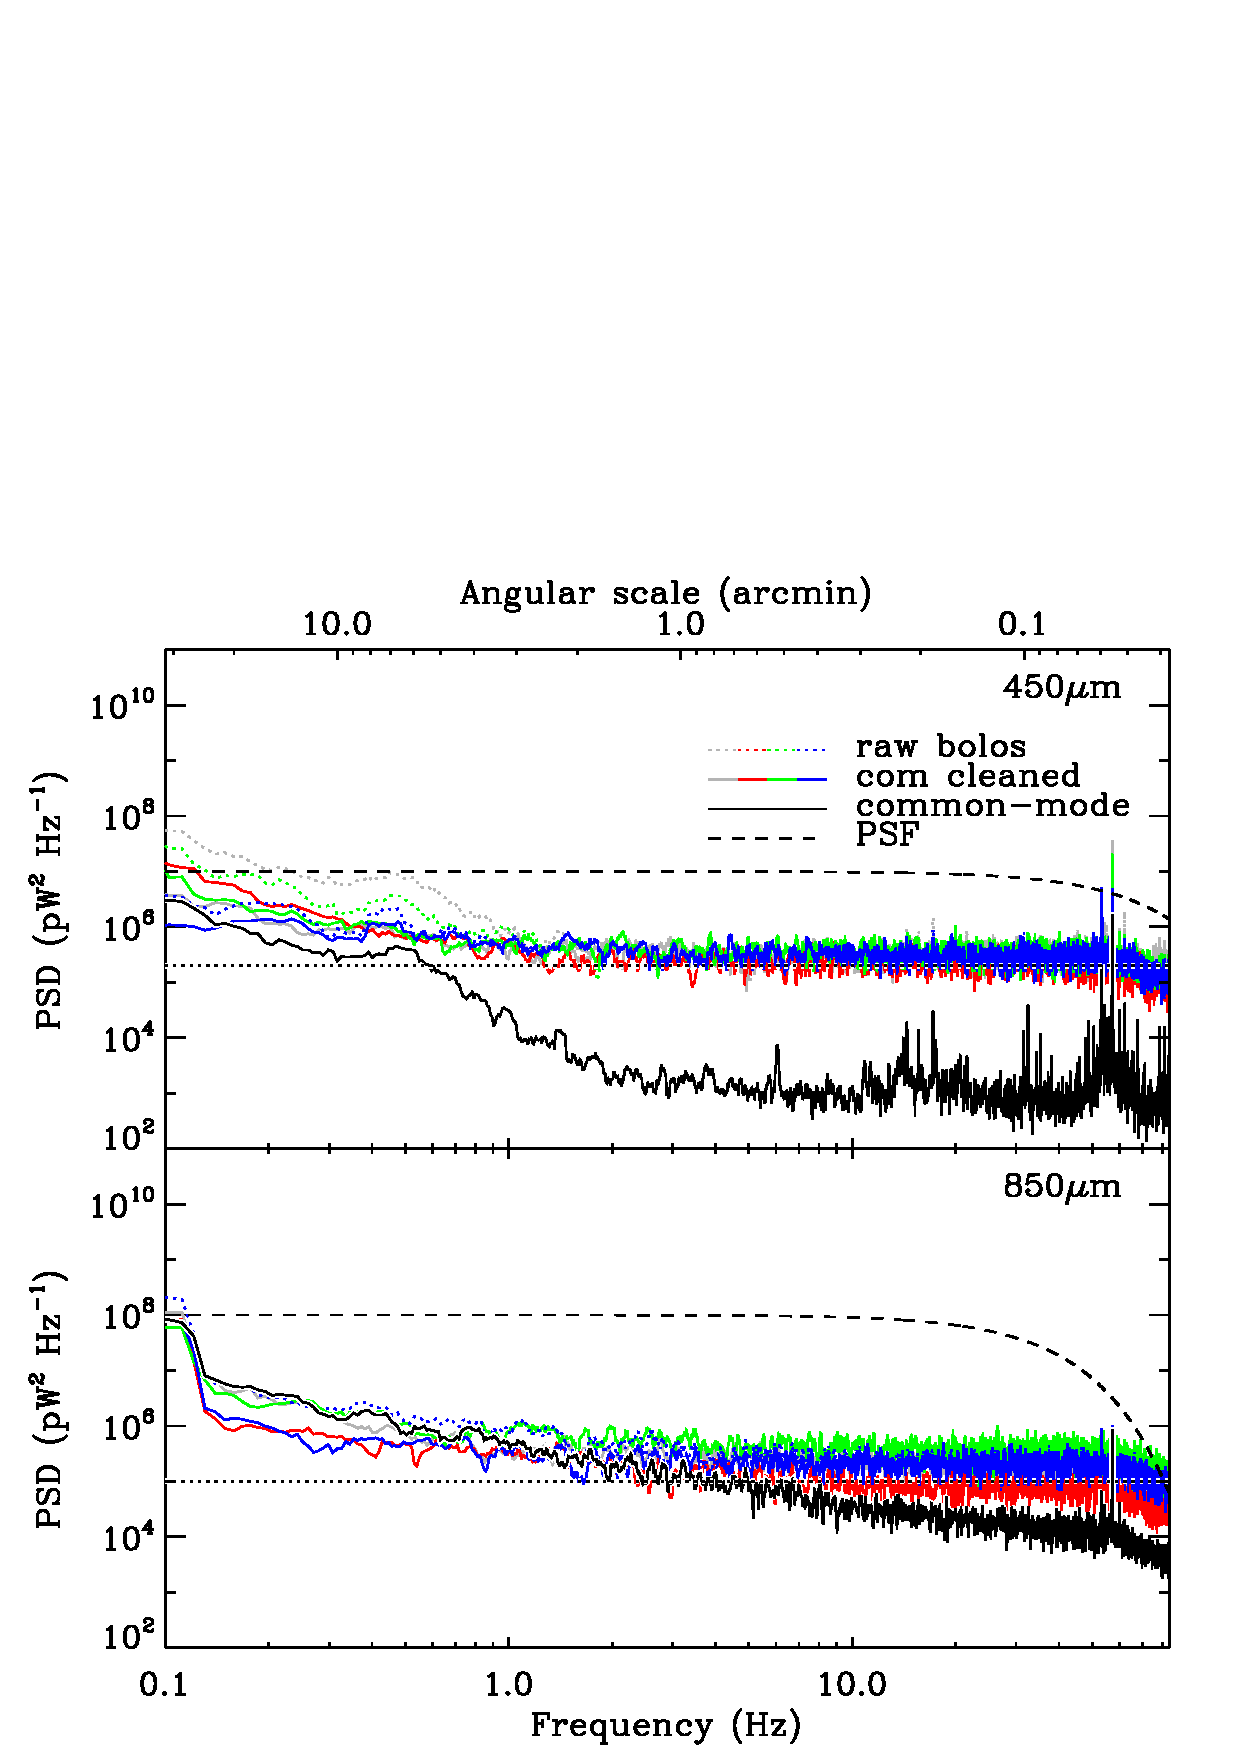
\includegraphics[width=\linewidth]{pspec.pdf}
\caption{Bolometer power spectral densities. Four representative
  bolometers have been selected from each sub-array, and the
  flat-fielded (but otherwise raw) PSDs are shown as coloured dotted
  lines (the blue signals are for the same time series as those shown
  in Fig.~\ref{fig:bolos_mix}). Horizontal dotted lines at $5 \times
  10^{-8}$ and $5 \times 10^{-9}$\,pW\,Hz$^{-1}$ at 450 and
  850\,\micron\ respectively, give the approximate white-noise
  levels. There are broad line features in the PSDs at both
  wavelengths above $\sim$35\,Hz. From $\sim$50\,Hz up to the Nyquist
  frequency, the gradual roll-off of the anti-aliasing filter is also
  evident.  At lower frequencies, the bolometer signals exhibit clear
  $1/f$ knees at approximately 2 and 4\,Hz at 450 and
  850\,\micron. The solid black lines are the PSDs of the common-mode
  signals at each wavelength, and the solid coloured lines show the
  PSDs of the bolometers once the common-mode is removed. These
  residual signals have significantly lower $1/f$ knees, approximately
  0.4 and 2\,Hz at 450 and 850\,\micron. Finally, the dashed black
  lines show the spectral shape produced by a point source, assuming
  that the telescope is slewing at 200\,arcsec\,sec$^{-1}$ (typical
  for S2SRO); for reference, the top horizontal axis shows the
  conversion from frequency to angular scale. We can see that the line
  features may add significant noise on the scale of the PSF. We also
  see that, for this scan velocity, the low-frequency noise begins to
  dominate on scales of approximately 8.3 and 1.7\,arcmin; these scales
  are comparable to the array footprint.}
\label{fig:pspec}
\end{figure}

The dotted coloured lines show the PSDs for raw, though flatfielded
data. At each wavelength, there is a clear $1/f$ knee at a few Hz,
followed by a predominantly white spectrum punctuated by line features
above $\gsim 30$\,Hz, and finally roll-off caused by the anti-aliasing
filter above $\gsim 70$\,Hz. As indicated in the previous section, the
correlation between the low-frequency components of the different
bolometer signals is large. The solid black lines in
Fig.~\ref{fig:pspec} indicate the PSDs of the common-modes
$\mathbf{c}(t)$ at each wavelength, which reproduce most of the
low-frequency structures, as well as the high-frequency line
features. The $\mathbf{c}(t)$ otherwise drop substantially below the
individual bolometer PSDs at high-frequency as expected if the
bolometers are dominated by un-correlated white noise. Finally, we
note that the amplitudes and slopes of the $\mathbf{c}(t)$ are
similar at both 450 and 850\,\micron. However, since the
450\,\micron\ white noise is larger than at 850\,\micron\ (shown
approximately by the horizontal dotted lines), the $1/f$ knee occurs
at a \emph{lower} frequency at 450\,\micron.

Next, the common-mode signals are fit to each bolometer time series
and removed as in Fig.~\ref{fig:bolos_mix}, and the resulting PSDs are
shown as solid coloured lines. In this example, the residual signals
have $1/f$ knees significantly lower than in the raw PSDs.

For reference, the top horizontal axis has been converted to angular
scale assuming a scan velocity of 200\,arcsec\,sec$^{-1}$ which was
typical of the S2SRO observations. The power spectra of the PSFs in
each band (arbitrary normalized to peak values of $10^{-6}$ and
$10^{-7}$\,pW$^2$\,Hz$^{-1}$ at 450 and 850\,\micron\ respectively)
are also showed as dashed lines for this assumed scan velocity showing
that the smallest features resolvable by the telescope may be slightly
affected by the excess noise in the line features. At the lower
frequency end, the $1/f$ noise dominates at scales $\gsim 2$\,arcmin
in the raw data and $\gsim 10$\,arcmin in the common-mode cleaned data
at 450\,\micron, and at scales $\gsim 1$\,arscmin in the raw data and
$\gsim 2$\,arcmin in the common-mode cleaned data at 850\,\micron.

\subsubsection{Principal component analysis}

\begin{figure*}
\centering
\includegraphics[width=\linewidth]{pca.pdf}
\caption{The first six modes from a principal component analysis of
  the combined 450 and 850\,\micron\ time-series bolometer data.}
\label{fig:pca}
\end{figure*}

\subsubsection{Sky noise}
Do we even see sky noise? Can show some results for the combined 450
and 850\,\micron\ joint PCA analysis.

\subsubsection{Magnetic field pickup}
Show that it occasionally appears in the dark squids.

\subsubsection{Line features}

The power spectra also show some narrower line features (many
correlated across the array). Even though we largely ignore them worth
some mention.

\begin{figure*}
\centering
\includegraphics[width=\linewidth]{pca.pdf}
\caption{The first six modes from a principal component analysis,
  ordered by decreasing significance, of the combined 450 and
  850\,\micron\ time-series bolometer data. For each component, the
  top plot shows the time series of the eigenvector, normalized by its
  \rms. The bottom coloured panels show the eigenvalues for the
  bolometers at each wavelength (the amplitude of the eigenvector in
  the time series). For reference, both the mean, $\bar{\lambda}$, and
  \rms, $\lambda_\mathrm{rms}$, eigenvalues for the bolometers in each
  subarray are also shown. The first two components have comparable
  amplitudes, and dominate by at least a factor of 10 any other
  components of the time series. We suspect that they are caused by
  atmospheric variations (expected to be brighter at 450\,\micron),
  and fridge oscillations (expected to be comparable at each
  wavelength). However, the two eigenvectors do not necessarily map
  directly to these physical sources under this interpretation; rather
  they are two \emph{different} linear combinations of the underlying
  physical signals that give rise to statistically uncorrelated
  components. The third component accurately reproduces an apparent
  data-acquisition glitch that appears only at 450\,\micron\ (see
  Section ???). The fourth component is a ...\,Hz line feature only
  observed in column 15 of the 450\,\micron\ subarray. The fifth
  component shows a series of steps and glitches that appear
  predominantly along the bottom-left edge of the 850\,\micron\
  subarray where the bolometers are only tenuously locked. Finally,
  the sixth component is degenerating into a less significant, and
  more randomly scattered signal across the focal plane. Subsequent
  components follow this trend, and would generally be kept in a
  PCA-cleaning procedure.}
\label{fig:pca}
\end{figure*}

%------------------------------------------------------------------------------
\section{The SMURF Algorithm}
\label{sec:algorithm}
%------------------------------------------------------------------------------

\begin{itemize}

\item Describe the bolometer signal model, and with the help of a flow-chart
show the basic procedure that SMURF follows.

\item Discuss SMURF configurability

\item Some sort of proof/demonstration showing why the algorithm works

\item Discuss performance (execution time, memory, disk usage etc.)

\item Where do you get SMURF/starlink, usage of NDF

\item Talk about pipeline?

\end{itemize}

We express the signal observed by the $i$th bolometer as a function of time,
\begin{equation}
\mathbf{b}_i(t) = g_i[\mathbf{e}_i(t) \mathbf{a}_i(t) + \mathbf{n}_i(t)]
\end{equation}
where $\mathbf{a}(t)$ is the time-varying signal produced by scanning
the telescope across astronomical sources, $\mathbf{e}(t)$ is the
time-varying extinction, which is a function of the telescope
elevation and atmospheric conditions, and $\mathbf{n}_i(t)$ represents
sources of noise. The two terms in square brackets, as written, have
units of power delivered to the detectors (pW). The scale factor $g_i$
converts this effective power to the digitized units recorded on disk
(DAC), and in this formulation is assumed to be constant in time.

In practice, $g_i$ is further factored into two components: $g_i = r_i
d$. The responsivity, $r_i$, gives the change in current as a function
of power fluctuations (A\,pW$^{-1}$). There is then a final (and
constant across all bolometers) conversion factor from current to DAC
units, $d$ (DAC/A).

As for the noise, $\mathbf{n}_i(t)$, we break it down into several
components,
%
\begin{equation}
  \mathbf{n}_i(t) = \mathbf{n}^\mathrm{w}_i(t) + \mathbf{n}^\mathrm{f}_i(t) +
  \mathbf{n}^\mathrm{c}(t),
\end{equation}
%
where $\mathbf{n}^\mathrm{w}_i(t)$ is uncorrelated white (thermal)
noise, $\mathbf{n}^\mathrm{f}_i(t)$ is low-frequency noise that is
\emph{not} correlated from bolometer-to-bolometer, and
$\mathbf{n}^\mathrm{c}(t)$ is a (predominantly low-frequency)
correlated or \emph{common-mode} component.

The primary goal of map-making is to model and remove
$\mathbf{n}^\mathrm{f}_i$ and $\mathbf{n}^\mathrm{c}$ from the
time-series. By re-gridding the remaining data we can then hope to
approach the theoretical noise limit in the map.

\begin{figure}
\centering
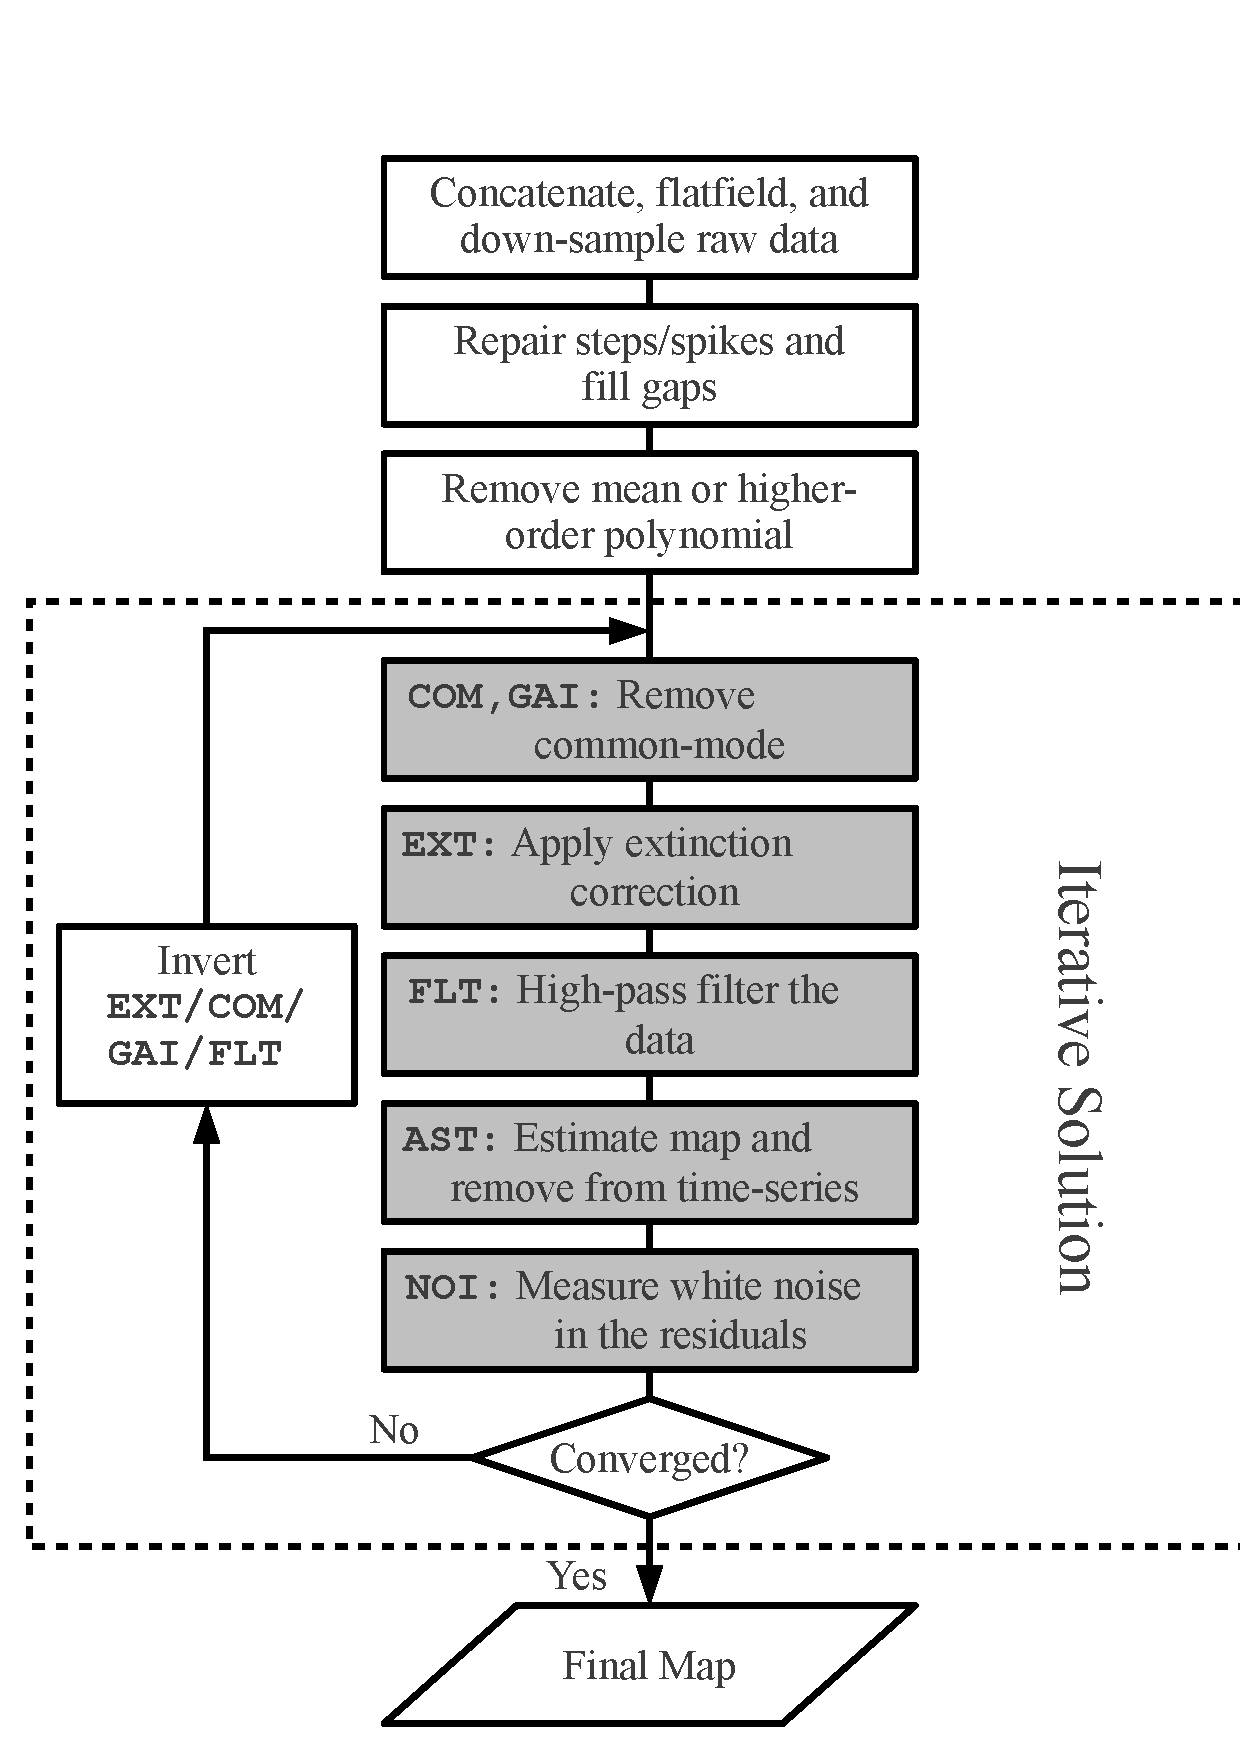
\includegraphics[width=0.75\linewidth]{dimm.pdf}
\caption{Typical map-making algorithm. Raw data (stored in multiple
  files) are read and concatenated into continuous time series. A
  pre-processing stage repairs DC steps, applies a flatfield
  correction, and identifies and removes the noisiest bolometers. The
  iterative portion then begins: estimating and removing the
  common-mode signal; applying the extinction correction; high-pass
  filtering to remove residual independent low-frequency noise;
  estimating the map by re-gridding the data; and finally measuring
  the noise in the residual time series. If the \rms\ has converged,
  the final map is written to disk. Otherwise any multiplicative
  factors that may have been applied to the data are inverted (e.g.,
  extinction correction and relative gains measured during the
  common-mode calculation), and each additive component is added back
  into the time series and re-estimated in turn.}
\label{fig:dimm}
\end{figure}

%-------------------------------------------------
\subsection{Model components}
%-------------------------------------------------

Give details about each model component, roughly in the order they are
calculated.

\subsection{Common-mode estimation}

DSB

We estimate the common-mode, remove it from the time series, use it to
flag bad bits of data, check for time-varying bolometer
responsivities... what doesn't it do?!

\subsection{Iterative filtering}

EC

The FFT filter can do high/low-pass filtering. We can also do notches
and whitening.

TJ

We also have the SMO filter that's useful for very short scans
because edge effects don't matter so much. Two sorts - median which is
more robust, or mean which is more accurate.


\subsection{Noise estimation}

Measure a white noise level from the power spectrum for each detector
to use as a weight.

\subsection{Map estimation}

In the map, use weighted standard error to estimate noise. This is
accurate for a single pixel, but there is still spatially correlated
noise in the maps which we can show with some figures.

\subsection{Model degeneracies}

Introduce the topic of model degeneracies here, but defer their
solution to the example sections.

%-------------------------------------------------
\subsection{Data cleaning}
%-------------------------------------------------

Since we can do most of this stuff either as a pre-processing step or
iteratively, I thinks this goes in a generic-sounding subsection. This
can go here, or perhaps earlier?

\subsubsection{Time-domain de-spiking}

DSB

\subsubsection{Step correction}

DSB

\subsubsection{Gap filling / apodization}

DSB

Discuss gap filling, ``new'' window function method, also apodization
and start/end polynomial continuity stuff. Should reference CMB
literature -- in particular look at \citet{stompor2002}.

\subsubsection{Flatfields}
\label{sec:flatfields}

TJ

Discuss heater ramps, normalizing off the common-mode signal
amplitude, astronomical sources, and the internal flatfield source.

\subsubsection{Additional bad bolometer rejection}

TJ

Measuring the noise power spectra and throwing away outliers. Data
flagged bad by the DA system.

\subsubsection{Map-based despiking}

EC

%------------------------------------------------------------------------------
\section{Examples}
\label{sec:examples}
%------------------------------------------------------------------------------

\subsection{Point source}
Reduce a calibrator. Describe the use of a zero mask around the
source. Compare with \citet{wiebe2009} who used the same method to
constrain a maximum-likelihood map with poor cross-linking.

\subsection{Deep blind survey}
Heavy initial filtering, and only iteratively solve for map and
common-mode with edge constraints.


\subsection{Bright extended emission}
The hardest thing to do with SCUBA-2 at the moment. Try to generate a
source/background mask to assist the map solution based on thresholds
in \snr. Compare with BOLOCAM stuff.

%------------------------------------------------------------------------------
\section{Summary and future work}
\label{sec:summary}
%------------------------------------------------------------------------------

\scuba\ is being re-commissioned. Maybe we will have some initial data
on fridge performance? If both it, and sky noise are relatively
well-behaved, might be able to restrict filtering to lower frequencies
and get larger-scale structures.

Larger array footprint also helps.

Talk about potential of Pascale et al. method to get closer to
max-likelihood map solution (handle maps at constant scan angles with
weights in Fourier space separately).

%------------------------------------------------------------------------------
\section{Acknowledgements}
%------------------------------------------------------------------------------


%------------------------------------------------------------------------------
\bibliographystyle{mn2e}
\bibliography{mn-jour,refs}
%------------------------------------------------------------------------------

%------------------------------------------------------------------------------
\appendix
\section[]{This is an appendix}
%------------------------------------------------------------------------------


\end{document}
